%
% exemplo genérico de uso da classe iiufrgs.cls
% $Id: iiufrgs.tex,v 1.1.1.1 2005/01/18 23:54:42 avila Exp $
%
% This is an example file and is hereby explicitly put in the
% public domain.
%
\documentclass[cic,tc]{iiufrgs}
% um tipo específico de monografia pode ser informado como parâmetro opcional:
%\documentclass[tese]{iiufrgs}
% monografias em inglês devem receber o parâmetro `english':
%\documentclass[diss,english]{iiufrgs}
% a opção `openright' pode ser usada para forçar inícios de capítulos
% em páginas ímpares
% \documentclass[openright]{iiufrgs}
% para gerar uma versão somente-frente, basta utilizar a opção `oneside':
% \documentclass[oneside]{iiufrgs}
\usepackage[utf8]{inputenc}   % pacote para acentuação
\usepackage{times}              % pacote para usar fonte Adobe Times
\usepackage[alf,abnt-emphasize=bf]{abntex2cite}	% pacote para usar citações abnt
\usepackage{graphicx}          % para inserir imagens
\usepackage{booktabs}
%\usepackage{mathptmx}          % p/ usar fonte Adobe Times nas fórmulas

\graphicspath{ {images/} }

\title{Uma análise dos dados de queimada do INPE no Brasil (preliminar)}
\translatedtitle{Using \LaTeX\ to Prepare Documents at II/UFRGS}

\author{Braz}{José Henrique da Silva}
\advisor[Prof.~Dr.]{Schnorr}{Lucas M.}

% a data deve ser a da defesa; se nao especificada, são gerados
% mes e ano correntes
%\date{maio}{2001}

% o nome do curso pode ser redefinido (ex. para TCs)
\course{Curso de Graduação em Ciência da Computação}

% o local de realização do trabalho pode ser especificado (ex. para TCs)
% com o comando \location:
\location{Porto Alegre}{RS}

% palavras-chave
% iniciar todas com letras maiúsculas
%
\keyword{Formatação eletrônica de documentos}
\keyword{\LaTeX}
\keyword{ABNT}
\keyword{UFRGS}

%
% palavras-chave na lingua estrangeira
% iniciar todas com letras maiúsculas
%
\translatedkeyword{Electronic document preparation}
\translatedkeyword{\LaTeX}
\translatedkeyword{ABNT}
\translatedkeyword{UFRGS}

%
% inicio do documento
%
\begin{document}

% folha de rosto
% às vezes é necessário redefinir algum comando logo antes de produzir
% a folha de rosto:
% \renewcommand{\coordname}{Coordenadora do Curso}
\maketitle

% dedicatoria
\clearpage
\begin{flushright}
\mbox{}\vfill
{\sffamily\itshape
``If I have seen farther than others,\\
it is because I stood on the shoulders of giants.''\\}
--- \textsc{Sir~Isaac Newton}
\end{flushright}

% agradecimentos
\chapter*{Agradecimentos}
Agradeço ao \LaTeX\ por não ter vírus de macro\ldots

% sumario
\tableofcontents

% lista de abreviaturas e siglas
% o parametro deve ser a abreviatura mais longa
% A NBR 14724:2011 estipula que a ordem das abreviações
% na lista deve ser alfabética (como no exemplo abaixo).
\begin{listofabbrv}{SPMD}
	\item[API] Application Programming Interface (Interface de Programação de Aplicação)
	\item[CSV] Comma Separated Values (valores separados por vírgulas).
    \item[GMT] Greenwich Mean Time
    \item[INPE] Instituto Nacional de Pesquisas Espaciais
    \item[IBGE] Instituto Brasileiro de Geografia e Estatística
    \item[URL] Uniform Resource Locator (Localizador Uniforme de Recursos)
    \item[NOAA] National Oceanic and Atmosphere Administration
    \item[MODIS] Moderate Resolution Imaging Spectroradiometer
    \item[GOES] Geostationary Operational Environmental Satellite
    \item[AVHRR] Advanced Very High Resolution Radiometer
\end{listofabbrv}

% idem para a lista de símbolos
%\begin{listofsymbols}{$\alpha\beta\pi\omega$}
%       \item[$\sum{\frac{a}{b}}$] Somatório do produtório
%       \item[$\alpha\beta\pi\omega$] Fator de inconstância do resultado
%\end{listofsymbols}

% lista de figuras
\listoffigures

% lista de tabelas
\listoftables

% resumo na língua do documento
\begin{abstract}
Este documento é um exemplo de como formatar documentos para o
Instituto de Informática da UFRGS usando as classes \LaTeX\
disponibilizadas pelo UTUG\@. Ao mesmo tempo, pode servir de consulta
para comandos mais genéricos. \emph{O texto do resumo não deve
conter mais do que 500 palavras.}
\end{abstract}

% resumo na outra língua
\begin{translatedabstract}
This document is an example on how to prepare documents at II/UFRGS
using the \LaTeX\ classes provided by the UTUG\@. At the same time, it
may serve as a guide for general-purpose commands. \emph{The text in
the abstract should not contain more than 500~words.}
\end{translatedabstract}

% aqui comeca o texto propriamente dito

%%%%%%%%%%%%%%%%%%%%%%%%%%%%%%%%%%%%%%%%%%%%%%%%%%%%%%%%%%%%%%%%%%%%%%%%%%%%%%%

\chapter{Introdução}

O fogo é uma tecnologia que está presente há milênios no território que hoje é o 
Brasil, desde queimadas controladas pelo povo indígena Kayapó no cerrado para 
plantio ou caça, até incêndios iniciados por combustão espontânea em períodos de 
seca no sul da Amazônia. O uso do fogo pelos indígenas era controlado, levando em 
conta o clima atual e a vegetação a ser queimada, e restrito apenas 
a um período do ano, com o intuito de reduzir pragas e ajudar nas plantações 
\citep{leonel_2000}. [P0. O que é uma queimada/fogo] \par

Hoje as queimadas que mais chamam atenção estão diretamente ligadas ao processo de 
desmatamento e manejo de áreas agrícolas para o cultivo da monocultura de soja. O 
fogo também é a prática mais barata e rápida para limpar áreas inteiras para a 
pecuária bovina. Commodites agrícolas e carne bovina movem a economia do Brasil, 
que é o maior exportador desses produtos, e aumentam a pressão para o 
desmatamento de novas áreas na Amazônia \citep{fuchs_2020}. 
[P1. As queimadas hoje] \par

O Brasil ocupa a quarta posição no ranking de nações que mais emitem gases de 
efeito estufa por habitantes, segundo dados da United Nations Environment Programme 
(UNEP) de 2022. De acordo com o 
estudo, o valor absoluto se manteve estável desde 2010, e atingiu seu pico por 
volta dos anos de 2003 a 2004. Assim como a Indonésia, o que melhor explica a 
alta posição do Brasil neste ranking são as 
queimadas e o desmatamento da vegetação nativa. Olhando para os municípios do país, 
dos dez que mais poluem, oito deles estão localizados no bioma da amazônia e não 
possuem atividades industriais que justificariam esse valor.
[P2. queimadas e efeito estufa no Brasil] \par

\begin{figure}
    \caption{Emissões de gases do efeito estufa per capta de 1990 até 2020 (tCO2e/capita)}
    \begin{center}
        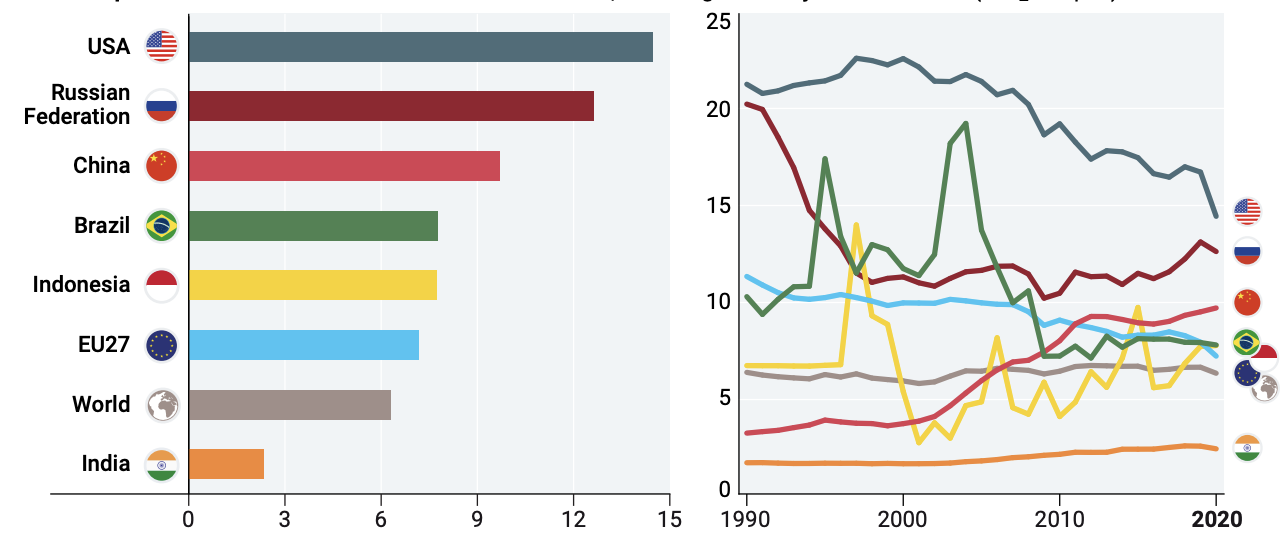
\includegraphics[width=35em]{emissoes_gee_per_capta}
    \end{center}
    \legend{Fonte: Emissions Gap Report 2022: The Closing Window}
    \label{fig:emissoes_gee_per_capta}
\end{figure}

Este trabalho se dedica a estudar e apresentar de forma concisa os dados de 
focos de queimadas disponibilizados pelo Instituto Nacional de Pesquisas Espaciais 
(INPE). O principal objetivo é tornar 
fácil o entendimento desses dados gerados a partir de imagens de satélites, sem a 
necessidade de um conhecimento prévio das técnicas de ciência de dados e 
sensoriamento remoto. O escopo de tempo das análises é limitado ao início 
de 1998, ano que iniciou a base aberta de queimadas, até o final de 2022.  
[P3. O que é o trabalho em si] \par

Os dados analisados neste trabalho foram obtidos a partir do DBQueimadas, 
Banco de Dados de Queimadas \url{www.inpe.br/queimadas/bdqueimadas},
que é um sistema desenvolvido pelo INPE e acessível de forma aberta por meio da web. 
Conta com mais de 300 milhões de pontos coletados desde o ano de 1998, 
provenientes de vários satélites \citep{setzer2019banco}. Ao disponibilizar os 
dados das queimadas o instituto possibilita que a sociedade retribua com pesquisas 
e fomenta novas abordagens ao problema das queimadas no Brasil, como é o caso 
deste trabalho. [P4. Fonte dos dados usados] \par

Durante o decorrer do documento são apresentadas diversas figuras, a maioria de 
construção do próprio autor, a fim de instigar a intuição do leitor para o 
tópico que está sendo abordado. De início, será abordado questões mais teóricas 
envolvendo caracteríscas dos satélites, suas produções de imagens e como são 
usadas para detectar um foco ativo de queimada. Após isso, .... 
[P5. Estrutura do documento] \par


%%%%%%%%%%%%%%%%%%%%%%%%%%%%%%%%%%%%%%%%%%%%%%%%%%%%%%%%%%%%%%%%%%%%%%%%%%%%%%%

\chapter{Fundamentação Teórica}

Neste capítulo, são apresentados alguns conceitos importantes para o entendimento 
de todo o trabalho. Para começar, serão formalizadas definições relacionadas às 
queimadas e como elas são monitoradas no Brasil. Na sequência, será feito uma 
sumarização dos principais satélites usados 
pelo INPE e suas características. Por fim, é dado uma visão geral de como as 
imagens brutas geradas pelos satélites são usadas para detecção de focos ativos.\par

\section{O monitoramentos das queimadas no Brasil}


[P0. definir uma queimada, focos detectados e área queimada] \par

[P0. Diferença entre foco detectado e área queimada] \par

[P1. Falar um pouco do INPE e suas divisões] \par

Dentro do site é possível gerar mapas,
tabelas, gráficos e exportar os dados sobre as queimadas no Brasil 
aplicando diferentes filtros. Todo o programa foi desenvolvido com 
ferramentas abertas, muitas delas criadas pelo próprio time de tecnologia da 
informação do INPE \citep{setzer2019banco}. 
[P2. Falamos sobre o programa DBQueimadas] \par

O Banco de Dados de Queimadas é um excelente caso de como os dados abertos podem 
ajudar a sociedade. Além do DBQueimadas, o INPE também 
disponibiliza para visualização e download, por meio da Divisão de Geração de 
Imagens (DGI) \url{www.dgi.inpe.br/catalogo/}, algumas imagens inteiras geradas 
pelos satélites que o próprio DGI captura e processa. 
[P3. importancia do dados abertos para a sociedade] \par

Para obter as imagens brutas dos satélites são necessárias antenas especiais que 
ficam em centros de recepção de dados. Com esse propósito, a DGI possui duas 
Estações de Recepção e Gravação (ERG) - a primeira 
em Cachoeira Paulista (SP) e uma mais recente em Cuiabá (MT). Na estação de SP, é 
feito o processamento de mais de 200 imagens de diversos satélites todos os dias, 
extraindo os dados de focos ativos de queimadas que alimentam o DBQueimadas. 
\citep{SiteDGI} [P4. Papel do DGI] \par

É em posse dessas imagens brutas que o INPE aplica algoritmos de detecção de 
focos de queimadas. No caso da detecção ser positiva, a posição exata (latitude e 
longitude) e a hora que a imagem foi gerada são
adicionadas aos dados como uma nova linha e disponibilizados pelo DBQueimadas. 
O INPE ainda coloca junto com as coordenadas da detecção mais alguns dados como 
risco de fogo, poder do fogo, precipitação e dados referentes a região do foco. 
A lista completa das colunas pode ser vista na Tabela \ref{table:inpeColumns}
 \cite{PerguntasFrequentesINPE}.
[P5. O que é uma observação nos dados] \par

\begin{table}[htbp]
\centering
\caption{Significado de cada coluna dos dados de queimada do INPE}
\begin{tabular}{@{}llp{9cm}@{}}
 \toprule
 \texttt{Atributo} & \texttt{Tipo} & Descrição \\
 \midrule
 \texttt{Id} & \texttt{string} & Identificador único registrado no banco \\
 \texttt{Latitude} & \texttt{double} & Graus decimais da latitude do centro 
                     do pixel de fogo ativo (valores de 90.0000 até -90.0000) \\ 
 \texttt{Longitude} & \texttt{double} & Graus decimais da longitude do centro 
                     do pixel de fogo ativo (valores de 180.0000 até -180.0000) \\  
 \texttt{DataHora} & \texttt{string} & Data a hora da passagem do satélite no fuso 
                     horário de Greenwich (GMT) \\   
 \texttt{Municipio} & \texttt{string} & Nome do município, de acordo com os dados 
                     do IBGE 2000 \\
 \texttt{Estado} & \texttt{string} & Nome do estado \\
 \texttt{Pais} & \texttt{string} & Nome do país \\  
 \texttt{Bioma} & \texttt{string} & Nome do bioma brasileiro, de acordo com 
                     dados do IBGE 2004 (para outros países o campo fica vazio) \\
 \texttt{Precipitação} & \texttt{double} & Valor a precipitação do dia até 
                     o horário da medida (-999 para valores inválidos) \\
 \texttt{DiasSCh} & \texttt{integer} & Dias sem chuva até a data da medida 
                     (-999 para valores inválidos) \\
 \texttt{RiscoFog} & \texttt{double} & Valor do risco de fogo previsto naquele dia 
                     (-999 para valores inválidos) \\
 \texttt{FRP} & \texttt{double} & Fire Radiative Power, MW (megawatts) \\
 \bottomrule
\end{tabular}
\legend{Fonte: O Autor com base em \citet{PerguntasFrequentesINPE}}
\label{table:inpeColumns}
\end{table}

[P7. Como é feito o calculo de área queimada pelo INPE] \par

\section{Os Satélites}

O INPE atualmente processa dados de vários satélites com características
distintas entre sí. Estão presentes nos dados desde satélites geoestacionários, 
como o GOES-12, que está a 29.400 km de distância da superfície 
\citep{GOES12Algo}, até satélites com óbitas polares, entre 700 a 900 km de altura.
[P0. Visao geral dos satelites] \par

Abaixo segue um resumo dos satélites usados pelos INPE desde o início da 
série histórica até final de 2022 \cite{EmbrapaSatelites}. 
Os que estão em funcionamento pleno atualmente são:
NOAA-20, NOAA-19, NOAA-18, GOES-16, Suomi NPP, AQUA, TERRA, MSG-03, 
METOP-B e METOP-C. [P1. Falar sobre os principais]\par

\begin{table}[htbp]
\centering
\caption{Características dos satélites usados pelo INPE}
\begin{tabular}{ @{}llllcl@{} }
  \toprule
  Nome    & Sensor & Resolução esp. & Órbita & Lançamento & Passagem \\
  \midrule
  METOP-C & AVHRR-3  & 1100m       & Polar   & 2018 & 21h \\
  NOAA-20 & VIIRS    & 500m        & Polar   & 2017 & 2h / 14h \\
  METOP-B & AVHRR-3  & 1100m       & Polar   & 2012 & 21h \\
  Suomi NPP & VIIRS  & 500m        & Polar   & 2011 & 2h / 14h \\
  NOAA-19 & AVHRR-3  & 1100m       & Polar   & 2009 & 2h / 14h \\
  NOAA-18 & AVHRR-3  & 1100m       & Polar   & 2005 & Variadas \\
  AQUA    & MODIS    & 1000m       & Polar   & 2002 & 2h / 14h \\
  NOAA-17 & AVHRR-3  & 1100m       & Polar   & 2002 & 21h \\
  NOAA-16 & AVHRR-3  & 1100m       & Polar   & 2000 & Variadas \\
  TERRA   & MODIS    & 1000m       & Polar   & 1999 & 11h / 23h \\
  NOAA-15 & AVHRR-3  & 1100m       & Polar   & 1998 & 5h / 17h \\
  TRMM    & VIRS     & 2000m       & Polar   & 1997 & Variadas \\
  NOAA-14 & AVHRR    & 1100m       & Polar   & 1994 & 21h \\
  NOAA-12 & AVHRR    & 1100m       & Polar   & 1991 & 2h / 15h \\
  GOES-16 & ABI      & 2000m       & Geoest. & 2016 & Não se aplica \\
  MSG-03  & SEVIRI   & 3000m       & Geoest. & 2012 & Não se aplica \\
  GOES-13 & GOES I-M & 4000m       & Geoest. & 2006 & Não se aplica \\
  MSG-02  & SEVIRI   & 3000m       & Geoest. & 2005 & Não se aplica \\
  GOES-12 & GOES I-M & 4000m       & Geoest. & 2001 & Não se aplica \\
  GOES-10 & GOES I-M & 4000m       & Geoest. & 1997 & Não se aplica \\
  GOES-08 & GOES I-M & 4000m       & Geoest. & 1994 & Não se aplica \\
  \bottomrule
\end{tabular}
\legend{Fonte: O Autor com base em \citet{EmbrapaSatelites}}
\label{table:satelites}
\end{table}

Cada satélite pode ter um sensor imageador, que gera imagens, com características
distintas. Neles são captados imagens não só no comprimento de onda da luz
visível (de 400nm a 700nm), mas também no infravermelho (de 780nm a 1mm). 
Suas medições são divididas em canais, que
variam em resolução espacial e espectral (intervalo de comprimento de onda). 
Geralmente o primeiro canal é dedicado à luz visível, entre o laranja e o 
vermelho, e com a maior resolução espacial possível para o sensor. Os outros 
canais utilizam diferentes intervalos do infravermelho e luz visível.
[P2. visão geral dos sensores e porque geram dados diferentes] \par

Com todas essas diferenças entre os satélites foi necessário estabelecer um 
satélite base, que ficou conhecido como Satélite de Referência. Ele é usado 
para estabelecer uma série temporal e permitir análise de tendência durante 
vários anos dos focos detectados para diferentes regiões. 
Este balizador precisa cobrir a área do país de forma
satisfatória, ou seja, sua órbita não deve distorcer os dados no geral. 
Além disso, resoluções dos sensores muito baixas, maiores de 1 km, tornam a 
análise dos focos pouca precisa. [P3. Satelite de referencia] \par

De 01/junho/1998 a 03/julho/2002 o satélite de referência utilizado foi o NOAA-12
com passagem no final da tarde. Depois desse período passou-se a utilizar o 
AQUA com passagem à tarde (chamado nos dados de AQUA\_M-T). O satélite AQUA 
já ultrapassou a data prevista de encerrar o funcionamento em muitos anos e 
será descontinuado em breve, quando isso acontecer o satélite Suomi NPP será o novo
balizador \citep{PerguntasFrequentesINPE}. [P3. Satelite de referencia] \par

Para finalizar, podemos observar na Figura \ref{fig:orbita2022-08-10} a passagem 
dos satélites no dia 10 de agosto de 2022, gerada a partir de 
dados do \url{https://celestrak.org/}. Os satélites podem levar 
vários dias para passar no mesmo local devido a características de sua órbita e 
podemos ter uma estimativa razoavelmente precisa de sua tragetória ao longo do 
tempo. Também é possível ver o satélite geoestacioário GOES-16, no norte 
do perú, representado com um ponto no gráfico. \par

\begin{figure}
    \caption{Órbita dos satélites no dia 10 de agosto de 2022}
    \begin{center}
        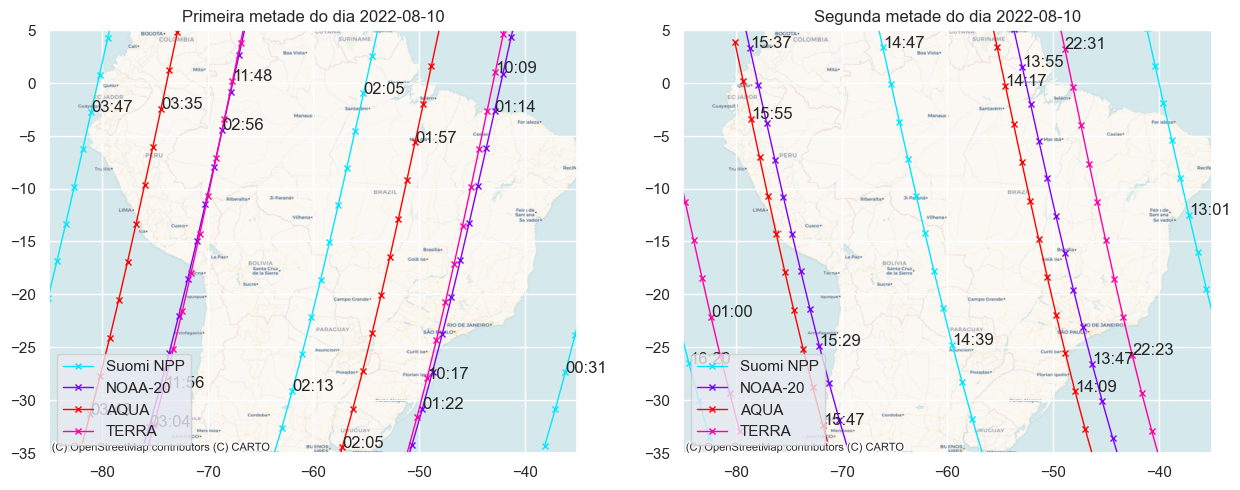
\includegraphics[width=35em]{orbita2022-08-10}
    \end{center}
    \legend{Fonte: O Autor}
    \label{fig:orbita2022-08-10}
\end{figure}

\section{Detecção dos focos de queimadas}

O algoritmo para identificação de focos ativos é específico para cada tipo 
de sensor. No geral, eles usam diferentes canais dos sensores dos 
satélites, entre a luz visível e o infravermelho, e podem ter comportamentos 
distintos dependendo se a imagem foi gerada à noite ou de dia. Podem também 
usar limiares dinâmicos, de acordo com a região do planeta, que são calculados com 
base em uma espécie de média das temperaturas nas regiões próximas ao longo dos 
dias. Além disso, é comum a aplicação de máscaras para eliminar regiões submersas, 
costeiras, deserticas e que estavam nubladas na hora da passagem. 
[P2. Visão geral dos algoritmos para detecçao] \par

Para o caso dos satélites TERRA e AQUA, que têm o sensor MODIS, o 
instituto mantinha seu próprio método de detecção, que produzia dados de 
maior confiabilidade \citep{PerguntasFrequentesINPE}. 
A partir de 2017 o INPE migrou toda a base de dados para o "Collection 6", 
algoritmo aplicado pela \textit{National Aeronautics and Space Administration} 
(NASA), marcando o início da chamada Base 2 de queimadas. Anteriormente, a NASA 
empregava o Collection 5, que gerava falsos positivos em clareiras florestais e 
falsos negativos para grandes queimadas obscurecidas por fumaça densa.
\citep{SCHROEDER2008}. [P3. Algoritmo empregrado pelo INPE] \par

O collection 6 .... \citep{GIGLIO2016} \par

Para detectar áreas queimadas, o instituto atualmente usa o produto AQ1km, 
desenvolvido em parceria com o Laboratório de Aplicações de Satélites Ambientais 
(LASA) \citep{SiteAQ1km} que ainda está em fase Provisória (ainda pode sofrer 
mudanças e não foi validada completamente). O produto é aplicados nos dados do 
sensor MODIS e, desta forma, usa os satélites AQUA e TERRA de forma 
concomitante \citep{libonati2015algorithm}. Uma vez que o AQUA foi lançado apenas 
em 2002, o produto só pode ser usados para dados a partir de 2003. \par

O AQ1km .... \citep{libonati2015algorithm} \par

%%%%%%%%%%%%%%%%%%%%%%%%%%%%%%%%%%%%%%%%%%%%%%%%%%%%%%%%%%%%%%%%%%%%%%%%%%%%%%%

\chapter{Trabalhos Relacionados}

[P1. falar sobre como os trabalhos relacionados podem ajudar a entender 
os dados] \par

%%%%%%%%%%%%%%%%%%%%%%%%%%%%%%%%%%%%%%%%%%%%%%%%%%%%%%%%%%%%%%%%%%%%%%%%%%%%%%%


\chapter{Metodologia}

A metodologia de pesquisa se dividiu em X etapas: Coleta e carregamento dos dados \par


\section{Coleta e carregamento dos dados}

Uma parte importante do processo foi coletar os dados do site DBQueimadas. 
Para exportar os dados utilizando o navegador de internet, é necessário 
preencher um formulário os campos de data inicial,
data final e um endereço de e-mail. O intervalo de tempo não 
pode exceder um ano. Também é possível aplicar filtros ainda mais 
detalhados como: continente, país, estado, município, satélite, bioma e 
unidades de conservação/terras indígenas. Após clicar em "Exportar", 
uma mensagem é enviada para o e-mail informado no formulário contendo link de 
download dos dados requisitados. O arquivo disponibilizado é um CSV compactado 
como um zip. [P1. Contextualizar como é a exportação de dados]\par

Apesar de ser um site com boas métrica e usabilidades, seria praticamente 
inviável baixar todos os dados do Brasil de forma manual. Nesse sentido, 
foi necessário entender quais eventos são disparados quando solicitamos 
os dados pelo site a fim de automatizar o processo de download. 
[P2. Motivar a abordagem automatizada] \par

Foi identificado que na verdade o site faz uma requisição GET para a API do 
DBQueimadas, localizada em 
\url{https://queimadas.dgi.inpe.br/queimadas/exportacaobdq/exportar}, 
passando nos parâmetros da URL os filtros informados pelo usuário, codificados 
em JSON. Além dos filtros, também é necessário informar o e-mail e o formato 
de arquivo desejado. Um exemplo de uso dessa API, por meio de uma invocação CURL, 
pode ser encontrado no \ref{anexo:usoApiInpe} [P3. Explicar como a api funciona]

A fim de automatizar o processo, foi desenvolvido um script em Python que 
solicita os dados referentes a 30 dias, totalizando 300 requisições de 1998 
até 2022. Com 
o intuito de não sobrecarregar os servidores do INPE, foi adicionada uma espera de 
um minuto a cada requisição. [P4. Falar sobre os scripts de coleta dos dados] \par

Para o processo ser concluído, ainda seria 
necessário fazer o download do arquivo por meio do link enviado por e-mail.
Lançou-se mão do Google Scripts, uma ferramenta que possibilita escrever 
programas simples, em uma liguagem parecida com JavaScript, e tem 
integração com os serviços do Google (como o Gmail). A partir dessa ferramenta
foi possível extrair o link de cada mensagem e finalmente salvar o arquivo
de forma automatizada. [P5. Processo de baixar os dados para o computador] \par

Todos esse processo de investigação e recuperação dos dados levou cerca de uma 
semana. Todos os arquivos baixados ocupam pouco mais de 4 Gigabytes de 
armazenamento em disco e somados tem exatamente 43.782.758 linhas. Ao final, eles 
foram recompactados em um único zip (450 Megabytes) e estão disponíveis 
em \url{https://bit.ly/3IgHIXH} para download de forma independete aos servidores 
do INPE. [P6. Conclusão do processo] \par

Também lançou-se mão dos dados públicos territoriais do Instituto Brasileiro de 
Geografia e Estatística (IBGE) com o intuito de gerar gráficos delimitados em 
municípios, unidades federativas e biomas. Todos os arquivos baixados estão em 
formato Shapefile, responsável por armazenar dados vetoriais geográficos. A 
biblioteca GeoPandas consegue ler e gerar gráficos a partir do Shapefile.
[P7. Dados territoriais] \par

%%%%%%%%%% Carregando os dados para análise e pre processamento

Para toda a análise dos dados foi utilizado algumas das ferramentas que integram o 
ecossistema Python para Data Sciente: NumPy, Pandas, Matplotlib. Além disso, 
algumas bibliotecas específicas para análise de dados geográficos: GeoPandas, 
Pysal, Xarray. Para a construção das visualizações e organização do código se 
optou pelo uso do Jupyter Notebook devido a reprodutibilidade das execuções. 
Todos os artefatos gerados podem ser obtidos em 
\url{https://github.com/josebraz/INPE-Queimadas} sobre a licença MIT. 
[P0. Visão das ferramentas utilizadas]\par

Os 300 arquivos das queimadas foram carregados para o Pandas e depois concatenados
em uma única estrutura de DataFrame. Houve a necessidade de converter o timezone 
das datas (que eram em UTC) para o timezone de Brasília, a fim de gerar gráficos 
de mais fácil entendimento para brasileiros. As colunas de texto foram convertidas 
para categorias, espécies de enumerações no Pandas, reduzindo o espaço ocupado 
de memória, uma vez que muitos valores acabavam se repetindo na mesma coluna. 
[P1. pre processamentos dos dados]\par

Como parte do pré-processamento dos dados, foi identificado regras de nomenclaturas 
especiais para alguns satélites. Para o AQUA (AQUA\_M-T e AQUA\_M-M) e TERRA 
(TERRA\_M-T e TERRA\_M-M), a primeira letra M representa o sensor MODIS e a última
letra indica em que período do dia foi a passagem do satélite, sendo M para Manhã 
e T para Tarde. Outros satélites como Suomi NPP, NOAA-19, NOAA-18, NOAA-16, NOAA-15 
e NOAA-12 também podem apresentar a última letra do nome sendo D para Diurno.
A partir do entendimento dessa regra de nomenclatura, foi possível criar uma nova 
coluna que informa o nome simplificado dos satélites, a fim de facilitar 
algumas análises. Em comparação com a coluna original dos satélites, que tinha 32 
valores possíveis, a nova coluna contém apenas 22 valores possíveis.
[P2. Explicar equivalencias entre os satelites] \par

A partir da coluna de nomes de satélites simplificada foi possível atribuir cores 
únicas para cada um (Figura \ref{fig:cores_satelites}), de forma a padronizar os 
gráficos e facilitar o entendimento.

\begin{figure}
    \caption{Cores escolhidas para cada satélite}
    \begin{center}
        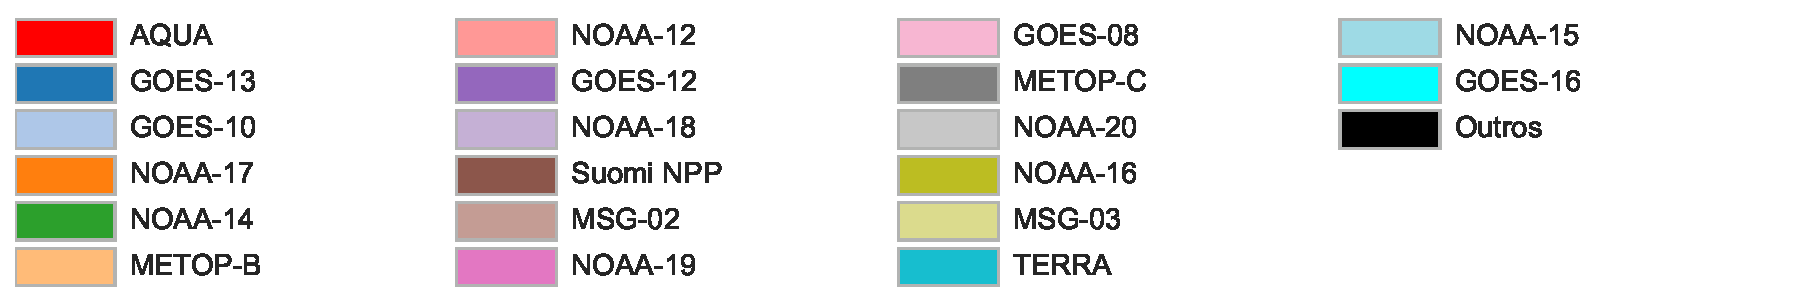
\includegraphics[width=35em]{cores_satelites}
    \end{center}
    \legend{Fonte: O Autor}
    \label{fig:cores_satelites}
\end{figure}


\section{Proposta de processamento de área queimada}





%%%%%%%%%%%%%%%%%%%%%%%%%%%%%%%%%%%%%%%%%%%%%%%%%%%%%%%%%%%%%%%%%%%%%%%%%%%%%%%

\chapter{Resultados e Discussão}



%%%%%%%%%%%%%%%%%%%%%%%%%%%%%%%%%%%%%%%%%%%%%%%%%%%%%%%%%%%%%%%%%%%%%%%%%%%%%%%


\chapter{Análise dos dados (ignorar)}

Neste capítulo, será feito uma análise dos dados de forma mais profunda, a 
fim de identificar padrões e formas de entendê-los usando ferramentas de 
visualização de dados.

\section{Uma visão geral}



Com relação aos satélites, e possível perceber a partir da Figura
\ref{fig:porcentagem_satelites} cinco satélites que mais identificaram  
focos de queimada, são eles: Suomi NPP, GOES-16, AQUA, NOAA-16 e TERRA. 
Todos eles estão 
ativos atualmente e com quantidades de coleta significativas em 2022. AQUA e TERRA 
são os mais antigos e possuem um sensor obsoleto. O GOES-16 é um satélite
geoestacionário, conhecido por gerar dados de forma mais frequente, geralmente 
detecta apenas queimadas maiores devido a sua posição distante da Terra. Suomi NPP e
NOAA-20 possuem um sensor que detecta 10 vezes mais focos que sensor MODIS. Por 
estar em atividade a mais tempo, o Suomi NPP gerou mais dados que o NOAA-20.
[P5. Mostrar gráficos da quantidade de coletas por satélites] \par

\begin{figure}
    \caption{Relação do montante dos dados por satélite}
    \begin{center}
        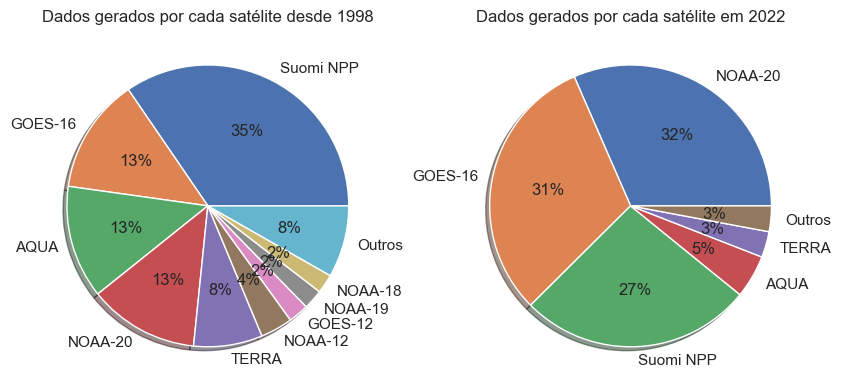
\includegraphics[width=35em]{porcentagem_satelites}
    \end{center}
    \legend{Fonte: O Autor}
    \label{fig:porcentagem_satelites}
\end{figure}

Saber em quais momentos os satélites passam também é importante para a análise. 
Os satélites polares passam duas vezes por dia no Brasil, variando o local 
exato da passagem de acordo com as características de sua órbita. Pela  
Figura \ref{fig:tempo_medidas_satelites} é possível observar esse comportamento 
empiricamente, em que as 5 primeiras linhas, que representam dados gerados por 
satélites polares, apresentam dois picos durante um período de 24 horas. Já para o  
caso dos geoestacionários (GOES-16), que ficam fixos em relação a uma posição 
na Terra, não se observou o mesmo padrão. 
[P6. Mostrar gráficos que indicam as horas das coletas] \par

\begin{figure}
    \caption{Amostragem por tempo de cada satélite}
    \begin{center}
        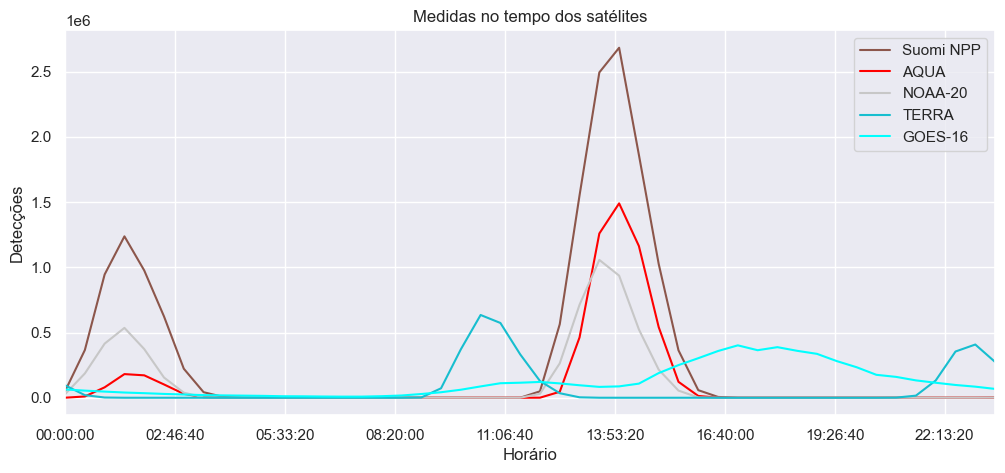
\includegraphics[width=35em]{tempo_medidas_satelites}
    \end{center}
    \legend{Fonte: O Autor, agrupando os dados de queimadas}
    \label{fig:tempo_medidas_satelites}
\end{figure}

\section{O que os dados gritam (padrões e tendências)}

Este capítulo vai dar uma primeira olhada nos dados, tentando extrair as 
informaç˜ões que mais chamam a atenção. É importante tomar um certo cuidado nessa 
análise geral, principalmente na escolha dos satélites. Se forem usados todos os 
satélites, provavelmente será contado um mesmo foco várias vezes, ou ainda, para um 
mesmo satélite polar, contar o mesmo foco nas duas passagens dele (de dia e a 
noite). Para evitar esse problema, será sempre usado o satélite AQUA com passagem a 
tarde (AQUA\_M-T) que é o satélite de referência. \par

A partir de uma análise quantitativa dos dados com relação ao tempo de cada medida,
exposto na Figura \ref{fig:quantitativo_geral}, podemos identificar uma grande 
sazonalidade, sempre tendo picos entre os meses de agosto e setembro. Desde o 
início da série, o mês que mais teve focos detectados foi setembro de 2007. 

\begin{figure}
    \caption{}
    \begin{center}
        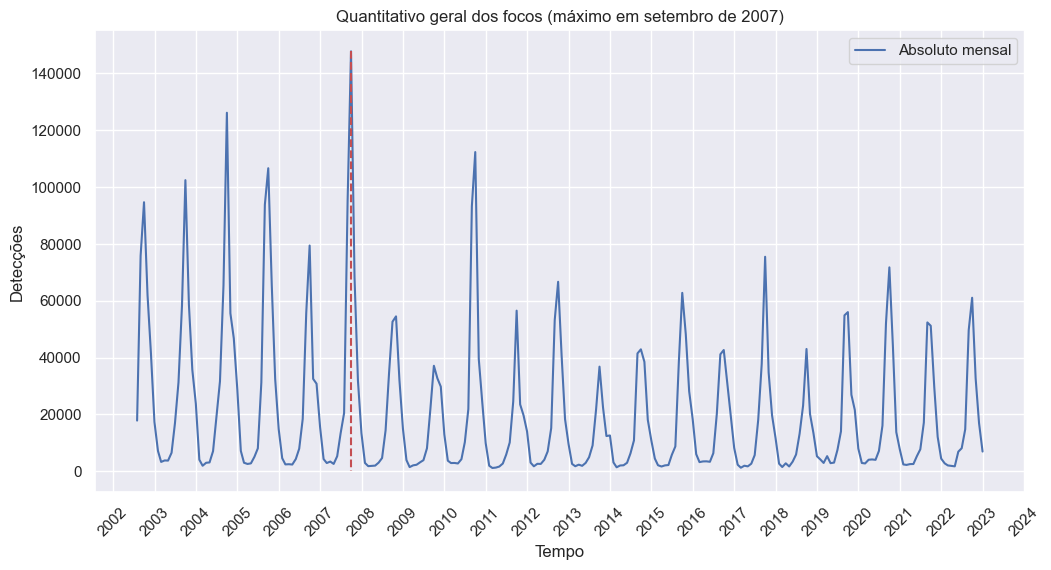
\includegraphics[width=35em]{quantitativo_geral}
    \end{center}
    \legend{Fonte: O Autor, agrupando os dados de queimadas por tempo}
    \label{fig:quantitativo_geral}
\end{figure}


P1. Fazer análise preliminar dos dados gerando alguns gráficos \par
P2. Gráficos geral do brasil com os focos de queimadas totais \cite{geographicDataSciencePython} \par


%%%%%%%%%%%%%%%%%%%%%%%%%%%%%%%%%%%%%%%%%%%%%%%%%%%%%%%%%%%%%%%%%%%%%%%%%%%%%%%

\chapter{Considerações Finais}

%%%%%%%%%%%%%%%%%%%%%%%%%%%%%%%%%%%%%%%%%%%%%%%%%%%%%%%%%%%%%%%%%%%%%%%%%%%%%%%


\bibliographystyle{abntex2-alf}
\bibliography{biblio}

\end{document}
